
\ChapterWithSubtitle{Evaporation and Clouds}{Show me my silver lining}
%\chapter{Heating by Radiation}

%%%%%%%%%%%%%%%%%%%%%%%%%%%%%%%%%%%%%%%%%%%%%
\section*{Equipment List}

\begin{multicols}{2}   % change 2 -> 3 for three columns
\begin{equipment}
\item Ruler
\item Hygrometer
\item Digital Thermometer
\item Ulanzi light / flashlight
\item 250 mL beaker (2)
\item 500 mL beaker 
\item Cloud chamber kit (cube with tube, felt, alcohol, caulk, baking tray, black vinyl, uranium rock)
\item Tall cloud jar w/ metal bowl for lid
\item Short cloud jar w/ glass bowl for lid
\item Dry ice chunk (instructor-provided)
\item Regular ice (in cooler)
\end{equipment}
\end{multicols}


%%%%%%%%%%%%%%%%%%%%%%%%%%%%%%%%%%%%%%%%%%%%%
\section{Introduction and Definitions}

\subsection{Atmospheric pressure and a warm-up experiment}

We have read that the the average atmospheric pressure at sea level on the Earth is about one kilogram force-equivalent per square centimeter of area ($\unit{2.2}{lb/\centi\meter^2} = \unit{14.2}{lb/in^2} = \unit{14.2}{psi} = \unit{101}{\kilo\pascal}$). This pressure is literally the weight of the column of air above us. Because liquid water is so much denser than air one can achieve an additional \unit{1}{atm} of pressure by submerging below just \unit{10}{\meter} of water\footnote{The pressure increase from the surface of a fluid to a depth $h$ is given by the equation $|\Delta P| = \rho g h$, where $\rho$ is the density of the fluid (\unit{1000}{\kilo\gram/\meter^3} for water) and $g \approx \unit{10}{\meter/\second^2}$ is the acceleration due to gravity.}.  Air pressure drops off exponentially with height in the atmosphere  with a {\em scale height} (distance over which it drops by a factor of $\frac{1}{\text{e}} \approx \frac{1}{3}$) of \unit{8}{\kilo\meter}, going to zero pressure --- a so-called {\em vacuum} --- in space.  The air pressure at Mount Everest base camp, 5,400~m above sea level, is about half what it is at sea level: $\sim \unit{50}{\kilo\pascal}$.\\[-6pt] 

\noindent{\bf Mini-experiment:} We do not ``feel'' the air pressure because it has the same value outside of our bodies (the air molecules beating against our skin) as it does internally (the water and blood molecules below our skin).  But there is a simple experiment we can do to observe its effects: evacuate the air in a soda can.  Together with your table of four students, put a small amount of water (less than  \unit{1}{\centi\meter} deep) into an empty soda can.  Heat this on a hot plate until the water has been rapidly boiling for a little while and, most importantly, the can is filled with water vapor\footnote{As we will ``see'' today, actual water vapor is invisible, so we only see its presence in the moments that it comes in contact with colder air and condenses into tiny liquid drops (what we call ``steam'').}.  By filling the can with pure water vapor, most of the air has been pushed out of the can.  If we could then rapidly condense the water vapor into liquid we would have an approximate vacuum inside the can (because the volume of {\em liquid water} associated to a can full of {\em water vapor} is miniscule).  Do this with your group by gently but quickly removing the can from the hotplate with tongs, and then turning it upside down and dunking it into a bowl of cold water.  Watch for any noticable effect on the can and document the experiment here.

\answerspace

\subsection{Phase transitions in air and partial pressure}

Last week in lab we boiled water in a 250~mL beaker.  We observed that, as expected for our classroom conditions at atmospheric pressure, boiling occured when the water reached 100$\degree$C.  Look back at the phase diagram for water that you marked up last week (Figure \ref{fig:07_phase-diagram-water}) and remind yourself why this was expected, i.e., following the horizontal line of $p = \unit{1}{atm}$ to the {\bf coexistence curve}  between liquid and vapor water.   You should have noticed in this experiment, however, that there was significant mass loss of liquid water prior to the ``boiling point.''  Mass of water dropped off rapidly once the water temperature reached 100$\degree$C (in some experiments at a rate of about \unit{3.5\times 10^{-2}}{\gram/\second}), but there was a measurable mass decline when the temperature was in the range 50--100$\degree$C  as well (a rate of about \unit{1.0\times 10^{-2}}{\gram/\second}). The reason for this is:
	%
	\begin{enumerate}[label=(\roman*)]
	\item The phase diagram we used last week pertains to {\em pure water}, i.e., liquid water in a closed container with only water vapor and ice.  This description applies to water in the bulk of the fluid, below its surface.  Once internal liquid water molecules reach 100$\degree$C, their intermolecular forces weaken and they are likely to separate from neighboring molecules to form water vapor instead, which then bubbles to the surface (``boiling'').
	\item Water molecules at the surface, however,  are exposed to air, so they are {\em not} in a ``pure'' liquid-vapor-water situation.  Generally air contains only some small percentage (precisely, a small {\em mole fraction}) of water vapor.  It turns out that\footnote{The physical reason for this result is due to the ideal gas law, where, as long as the densiities are quite low, all types of gas molecules treated as the identical non-interacting particles; so the liquid water at the surface only ``sees'' a low-density water-gas within the total air gas.} the same phase diagram can be used to determine the coexistence curve, but for pressure one must use the so-called {\bf partial~pressure} of water in air: 
		%
		\begin{equation*}
		e = f \times p_\text{atm} = \frac{n_{\, \text{H}_2\text{O}}}{n_{\, \text{H}_2\text{O}} + n_\text{dry air}} \times p_\text{atm}
		\end{equation*}
		%
	where $e$ is the variable\footnote{This is not the same ``e'' mentioned above in the ``scale height'' discussion; that was the exponential constant, or {\em Euler's number}, $\text{e} = 2.718\ldots$.} typically used for partial pressure, and $n$ is the variable for the number of moles, so $f$ is the {\em mole fraction of water in air}. Because the mole fraction of water in air is generally significantly less than one (on the order of 1\%), the partial pressure of water in air is significantly less than (about 1\% of) atmospheric pressure. 
	\end{enumerate}
	%
So, your boiling experiment was actually two separate experiments occuring at once: a pure-water phase transition occuring below the surface, and a liquid-to-vapor-in-air transition occurring at the surface.  Make a sketch of your boiling water beaker and point to the two different  water vapor pressures at the two different locations.  Sate the the variable names of these pressures and estimate their values roughly (using the ``1\%'' estimate given above).

\answerspace

\noindent We will do this more precisely in a moment, but quickly return to your phase diagram from last week  (Figure \ref{fig:07_phase-diagram-water}) to estimate the vaporization temperature for the water at the surface, where $e \approx 0.01 \times p_\text{atm}$.  Record this temperature value (as best you can read off that graph) here.

\answerspace[2cm]

\subsection{Relative humidity, absolute humidity, and dew point temperature}

\noindent The vaporization temperature for liquid water in contact with air is called the {\bf dew point temperature}.  Let's determine this value more carefully.  First look up the ``current conditions'' on a weather page (e.g., search for ``NWS 7-day grand rapids'') and record the current temperature, the {\bf relative humidity} (expressed as a percentage), and the dew point temperature. [Note: If it is currently raining and/or the humidity is greater than $\sim85\%$, choose a different data point within the ``3 Day History'' when the humidity was lower.]

\answerspace[2cm]

\noindent Now examine the so-called {\bf psychrometric chart} shown in Figure \ref{fig:08_psychrometric-and-phase-diagrams}.  Use your temperature (horizontal axis) and relative humidity (curved lines labeled at top) values to determine the associated {\bf absolute humidity} (vertical axis), which is expressed here as a ratio of water mass to (dry) air mass:
	%
	\begin{equation*}
	\text{AH} = \frac{m_{\, \text{H}_2\text{O}}}{m_\text{dry air}}
	\end{equation*}
	%
To determine the partial pressure of water in air, we must find the mole fraction, $f$, from this quantity.  \underline{Let's derive the relationship between $\text{AH}$ and $f$ now.}  \\[-6pt]

\noindent (i) Recall that the number of moles of a gas can be expressed as $n = m / M$ where $m$ is the actual mass of the volume of gas and $M$ is the {\bf molar mass} of the gas (determined by summing the molar masses given on a periodic table for each of its component atoms).  Find $M$ for water and for dry air. Remember that water is $\text{H}_2 \text{O}$, and air is basically 80\% nitrogen ($\text{N}_2$) and 20\% oxygen ($\text{O}_2$), so $M_\text{air} = 0.8 M_{\text{N}_2} + 0.2 M_{\text{O}_2}$. 

\answerspace[6cm]

\noindent (ii) Now write out the {\em mole ratio}
	%
	\begin{equation*}
	r = \frac{n_{\, \text{H}_2\text{O}}}{n_\text{air}} \, ,
	\end{equation*}
	%
using the $n = m/M$ equation in both the numerator and denominator, and then simplify to express it in terms of AH (for now, don't plug in the number for the absolute humidity, just replace $m_{\, \text{H}_2\text{O}} / m_\text{dry air}$ with ``AH'').

\answerspace[6cm]

\noindent (iii) Write down the equation for the mole fraction of water in air
	%
	\begin{equation*}
	f =  \frac{n_{\, \text{H}_2\text{O}}}{n_{\, \text{H}_2\text{O}} + n_\text{ dry air}} \,.
	\end{equation*}
	%
We wish to express this in terms of AH.  To do so, you can first express it in terms of the mole ratio, by multiplying the numerator and denominator by $\frac{1}{n_\text{ dry air}}$. You should find that the mole ratio appears in two places.  Then you can use your expression from the prior step to write re-write the mole fraction in terms of the AH value (as well as a numerical value that depends on the molar mass values calculated above).

\answerspace[5cm]

\noindent \underline{Check your answers with your table mates and your instructor.} \\[-6pt]

\noindent Now: convert the AH value you found from the psychrometric chart into a mole fraction value\footnote{It is expressed in grams per kilogram, so if you write it instead as grams per grams (e.g., $\unit{7}{\,gram} / \unit{1}{\kilogram} = \unit{7}{\gram} / \unit{1000}{\gram} = 0.007$).}; plug that value in your derived equation for $f$; and calculate the partial pressure value, $e = f \times p_\text{atm}$, in units of atmospheres (atm).

\answerspace[4cm]

\noindent Finally, using the new phase diagram provided in Figure \ref{fig:08_psychrometric-and-phase-diagrams}, determine the vaporization temperature of water in air, given the partial pressure you determined.  Compare this to the dew point value in the weather report.

\answerspace[3cm]

\noindent  \underline{Questions:} You should find in the weather data, and in your calculated verification, that the dew point temperature is well below the air temperature.  What do you think are the implications of this fact?  What will happen if you spill water on the table?  What is the meaning of ``relative humidity,'' and what happens to the relative humidity as the air temperature decreases to the dew point?  How does the ``distance to the dew point'' (and the relative humidity) affect your body's ability to cool by perspiration?
	



%%%%%%%%%%%%%%%%%%%%%%%%%%%%%%%%%%%%%%%%%%%%%
%%%%%%%%         Psychrometric Chart and Phase Diagram        %%%%%%%%%%%
%%%%%%%%%%%%%%%%%%%%%%%%%%%%%%%%%%%%%%%%%%%%%
\newpage

\begin{figure}
\centering
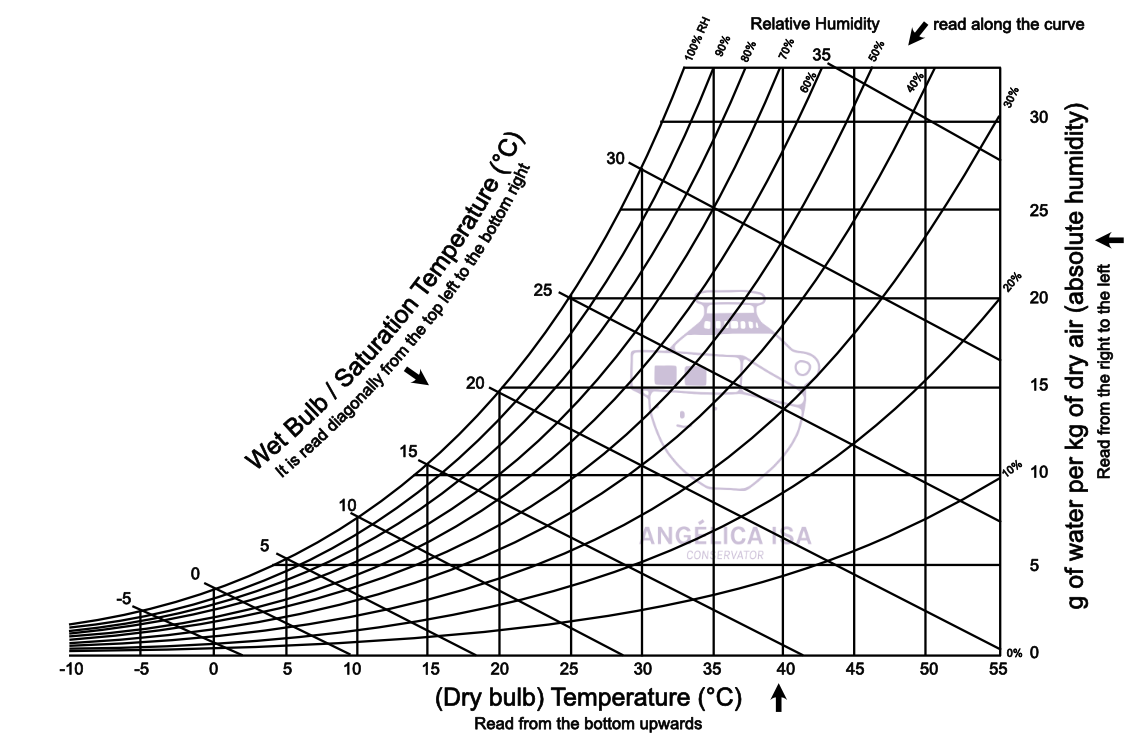
\includegraphics[width=0.95 \textwidth]{images/08_psychrometric_angelica-isa.png}\\
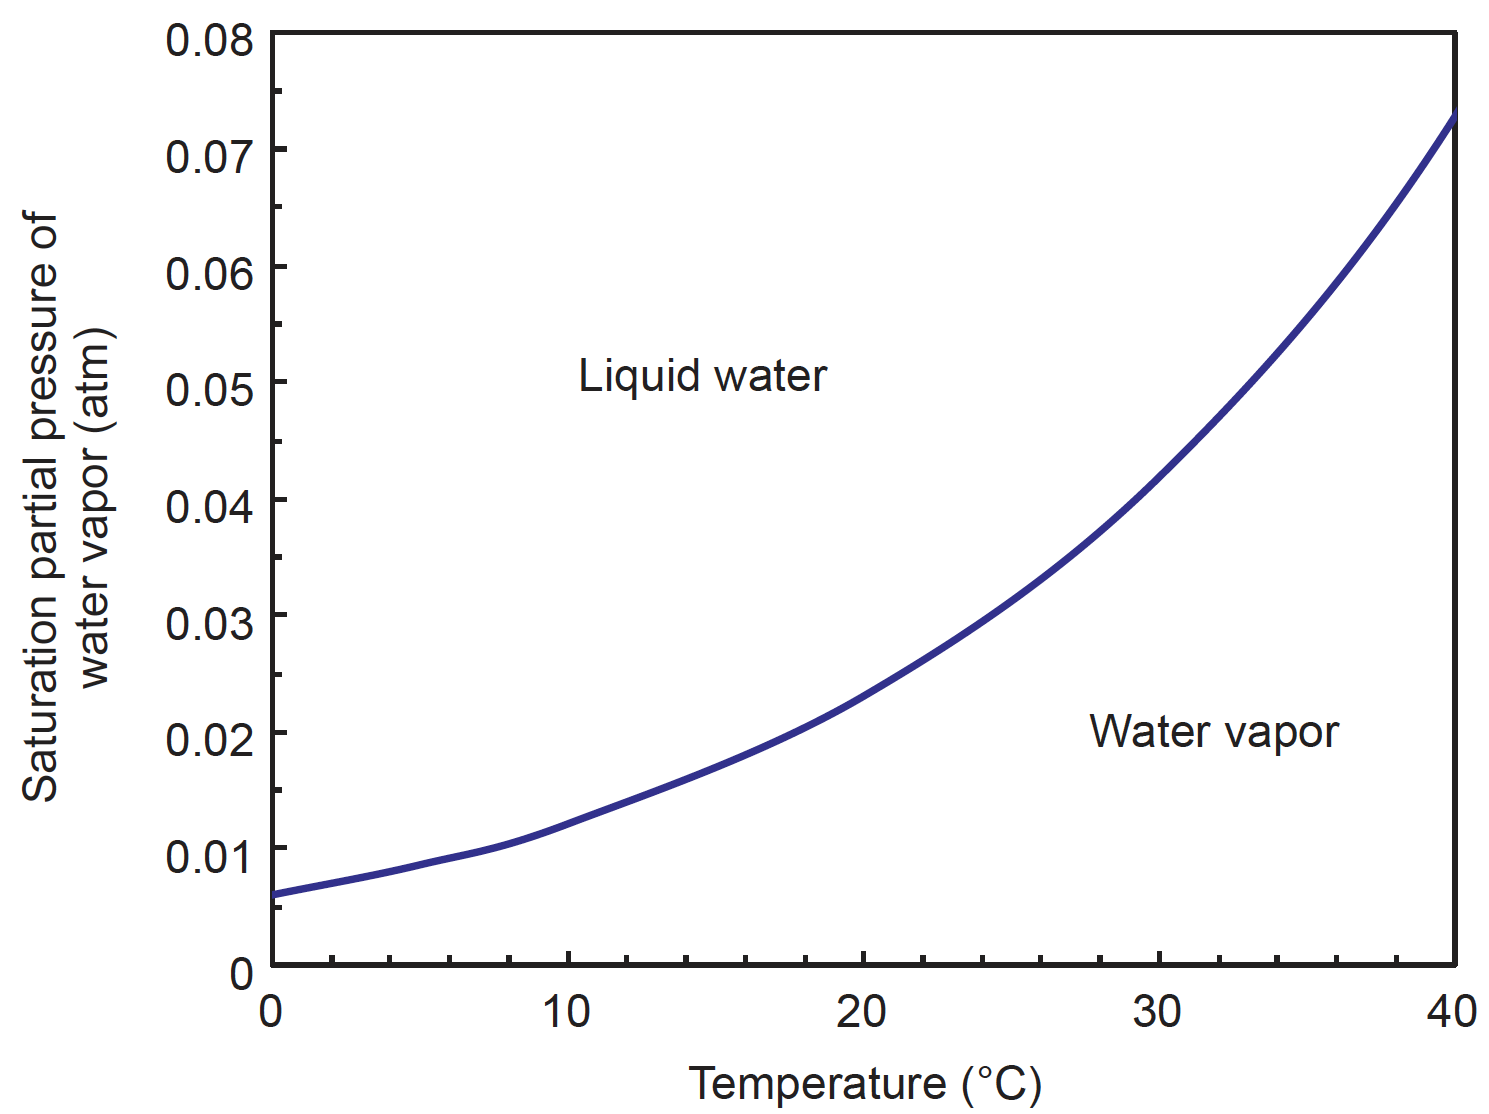
\includegraphics[width=0.95 \textwidth]{images/08_pressure-vs-temperature-clausius-clapeyron_mathez-fig-1-2_no-caption.png}
\caption{ \label{fig:08_psychrometric-and-phase-diagrams}
{\bf Top}: Psychrometric chart for water at standard pressure conditions $\unit{1}{atm} = \unit{101}{\kilo\pascal}$ (from angelicaisa.com). {\bf Bottom}: Phase transition coexistence curve for water near the triple point (from Mathez \& Smerdon).
}
\end{figure}



\newpage
%%%%%%%%%%%%%%%%%%%%%%%%%%%%%%%%%%%%%%%%%%%%%
%%%%%%%%%%%%%%%%%%%%%%%%%%%%%%%%%%%%%%%%%%%%%


%%%%%%%%%%%%%%%%%%%%%%%%%%%%%%%%%%%%%%%%%%%%%
\section{Experiments and Analysis}

{\bf \underline{Safety Notes}:} 
	%
	\begin{itemize}
	\item For the ``cloud chamber'' experiment, your instructor will provide you with a chunk of solid carbon dioxide (``dry ice'').  This is about $-80\degree$C and it will burn you if you touch it. So,  please {\bf use the thermal gloves to handle the dry ice} if you need to (but you probably won't need to handle it).
	\item Also for the cloud chambers, you will be provided with a small radioactive rock (containing uranium and other things).  As we will see, this emits ``alpha particles'' (helium nuclei). These particles are not able to penetrate your skin and are therefore safe.  However, you would not want to consume these rocks as the alpha particles could damage you internally.  So do not eat the radioactive rock, and also {\bf do not touch the radioactive rock without nitrile gloves}.  If you do happen to touch the rock, then wash your hands carefully.
	\item We can use smoke from a match to stimulate ``nucleation'' of clouds from the water vapor.  Be sure to keep your match strkes far separated from the isopropanol (alcohol), which is very flammable.
	\end{itemize}

\subsection{Observing the dew point and frost point}

We will not be performing our experiments outside, so we need to calculate the partial pressure of water for the conditions in this room.  Measure the temperature of the room with the IR thermometer gun (look at a bunch of objects that should be in thermal equilibrium with the air), and the relative humidity using the hygrometer.  Also give uncertainties for these measurments (and your rationale for these values).

\answerspace[3.5cm]

\noindent Use the process from the introduction, and your equation for $f$, to convert your relative humidity value to an absolute humidity (AH) and finally to a partial pressure, $e$, in atmospheres.  Then use the coexistence curve in the phase diagram (Fig \ref{fig:08_psychrometric-and-phase-diagrams}) to determine the vaporization temperature (the dew point) in this room.  Record the value and any intermediate calculations here.

\answerspace

\noindent Put some ``cold'' tap water in a 250~mL beaker; measure and record its temperature.  Then slowly add ice to the water to reduce its temperature.  Observe what happens to the outer walls of the beaker, noting the temperature(s) at which any changes occur.  Record your observations here and give an explanation for what is occuring.

\answerspace

\noindent If you examine the full phase diagram from last week  (Figure \ref{fig:07_phase-diagram-water}),  you see that the coexistence curve between liquid water and solid water is basically vertical, meaning it has the same transition temperature regardless of the pressure value.  What does this means for ``freezing of liquid water exposed to air'' (as compared to our discussion above of evaporation while boiling, pure water vs.\ surface water)?

\answerspace[3cm]  

\noindent Try to observe this {\bf frost point} by cooling your water further (this can be accomplished by adding salt to the water, since ``freezing point depression'' lowers the transition temperature within your beaker, allowing the water-salt-ice mixture to go below 0$\degree$C). Record any observations and temperature measurements.

\answerspace


\subsection{Drying your hands}

You are familiar with washing your hands and letting them dry off.  Let's try to quantify that experience, slightly.  Measure the temperature of ``cold'' water from the tap. Then run your hands under the water for a few seconds.  Turn off the water and shake off your hands five times to remove large water droplets.  Now wave your hands back and forth in the air in a regular motion while your partner times you with a stopwatch. Stop the timer when your palms are dry, as determined by your partner.  Repeat the whole experiment with ``hot'' water from the tap.   Record your temperatures, times, and observations here.


\answerspace

\noindent You likely found a measureable difference between the two cases. Why do you think that is the case? How can it be explained physically?

\answerspace


\subsection{An alcohol upside-down cloud}

Particle physicists use ``cloud chambers'' to observe the paths of particles in nuclear reactions (e.g., the break-up of atoms into smaller atoms by fission) and particle collision experiments.  We will build such a chamber using isopropyl alcohol (isopropanol).  The reason that alcohol is used is because it actually {\em does not} make clouds easily: it does not {\bf nucleate} as easily as other substances, meaning that vapor will remain vapor below the liquid-vapor transition temperature if there are no good ``seeds'' on which to form water droplets.  A {\bf cloud} is actually not composed of vapor, but is instead small liquid or ice droplets that have formed when vapor cools and condenses.  So, in the cloud chambers we will build (and that particle physicists use) the air is {\em super saturated} with alcohol and makes a ``cloud'' (the trail of tiny liquid particles) only when driven to nucleation by the ionization of air/alcohol from the passing nuclear decay particles (alpha particles, i.e., Helium nuclei).\\[-6pt]

\noindent {\bf Procedure:} 
	%
	\begin{itemize}
	\item Construct your cloud chamber by doing the following: (1) Fold a piece of felt in half and cut it so that the folded piece matches the base of the cubical box. (2) Attach the felt to inside bottom of the box using magnets. (3) Cover the bottom of the baking pan with black acrylic (4) Soak the felt with alcohol; it should be wet, but there should not be excess liquid in your box when you turn it upside down (if there is, pour that out). (5) Place a radioactive rock at the center of your upside-down baking sheet (your instructor will bring it over using gloves). (6) Turn your baking sheet upside down (acrylic side up); place a small radioactive rock on the center of the sheet (using gloves); and then place the cloud box upside-down onto the baking sheet. (7) Seal the bottom edge of the box to the baking sheet using caulk and the caulk spreader, all the way around the four edges.  (8) Place a chunk of dry ice (your instructor will bring it over using thermal gloves) on the corkboard mat and place the baking sheet  with box on top of the dry ice, so that the black ``floor'' of your box is cold.
	\item The clouds are best observed in a mostly dark space, using a flashlight. Look for ``streams'' of cloud emerging from the radioactive rock.  Try to take a video of it with your phone or the go-pro camera.  The particles should be leaving the rock with high velocity generating a straight-line cloud, which then sinks and floats away.  Can you catch an image straight-line cloud?
	\item As noted above, the alcohol does not nucleate well, so although its temperature is below the vaporization temperature (in the region near the dry ice base) it remains vapor (until the alpha particle causes an ionization trail).  You can force the alcohol to nucleate by lighting a match, letting it go out, collecting the smoke with the syringe, and then pumping smoke into the box through its tube.  Just a small amount of smoke should lead to a much larger volume of ``cloud.''  The smoke provides aerosol particles as nucleation sites.  Once you add the smoke, you will not likely see the radioactive emissions anymore.
	\end{itemize}
	%
Draw your setup and describe your observations.  

\answerspace[7cm]
	
\noindent Describe the entire process by which the clouds are formed here, starting with the liquid alcohol in the felt.  Make clear what is seen and what is invisible.

\answerspace[7cm]

\subsection{Cloud convection}

Now we will build clouds made of water vapor.  The reason the alcohol clouds were ``upside down'' (the alcohol was placed on the ceiling, the clouds formed down at the cold bottom layer) was because alcohol vapor is {\em more dense} than air and therefore sinks.  Water vapor, however, is {\em less dense} than air, so once formed it will rise in air. In our enviroment outside, water evaporates off of  lakes and oceans and then rises upwards.  When the temperature drops sufficiently, the water vapor (invisible) becomes liquid or ice droplets forming a cloud that can be seen.  In this experiment, we will partially fill a jar with warm water and then create a cold ``roof'' that is is a bit below 0$\degree$C. This actually perfectly matches the warm climate we experience at Earth's surface and the colder temperatures you would measure going vertically upward in the atmosphere.\\[-6pt]

\noindent {\bf Procedure:}
	%
	\begin{itemize}
	\item We will construct water vapor clouds in glass jars (either short or tall; you will have a chance to experiment).  The basic setup will be: warm tap water in the bottom of the jar; a bowl of salted-ice slurry\footnote{A {\em slurry} is a mixture of denser solids suspended in liquid, usually water; here we dissolve and suspend salt.} sitting on the lid; a flashlight to observe any convection; small amounts of added smoke to force nucleation and visible clouds.
	\item Create your salt-ice slurry by filling a 500~mL beaker with ice and adding a lot of salt.  Start stirring it vigorously and the ice will begin to melt forming a water-ice-salt mixture at the bottom.  You don't want too much water because you are relying on the the very cold (-20 to -10$\degree$C) ice to bring the mixture below the freezing point of water. So try to avoid adding water.  Use your thermometer to monitor the temperature of your slurry.  You can pour out water and add ice to keep it getting colder.  You should be able to easily produce a slurry of -10$\degree$C or lower.
	\item Get warm or hot water ($\sim40\degree$C) from the tap and fill the jar with about an inch of water.  
	\item Put slurry in the small glass bowl and fit it into the open lid of the jar.
	\item Turn off the lights and observe with a flashlight.  You should start to see ``convection'' rolls as the water vapor evaporates off the warm water surface, rises quickly and then condenses and cools near the top, falling as colder air or vapor.  
	\item Like the alcohol cloud chamber, you can force nucleation by adding some aerosol particles.  Light a match and blow it out, lift the bowl and wave a small amount of smoke into the jar.  Again you should see more cloud formed than just the smoke that you added, since the smoke acts as a nucleation site for cloud (as well as being visible itself as a tracer). Try to add a small amount of smoke at first.  You can always blow out your jar and re-start.
	\end{itemize}
	%
Draw your setup and describe your observations.  

\answerspace[7cm]
	
\noindent Describe the entire process by which the clouds are formed here, starting with the liquid water in the base of the jar.  Make clear what is seen and what is invisible.

\answerspace[7cm]


\subsection{Less convective clouds}

Since these water-vapor cloud jars are easy to make and adjust, we can try to vary the parameters to alter the conditions of the cloud formation and equilibrium.  The conditions for the previous setup included a large temperature gradient between the liquid ($\sim40\degree$C) and the cold ceiling ($\sim-15\degree$C).  This large difference should have led to a rapid rolling convection of the atmosphere in the jar.  Here we would like to adjust the setup to try to obtain clouds with less convection, i.e., a more stable layer of clouds.  \\[-6pt]

\noindent Discuss the relevant temperatures and heights involved in the formation of clouds in our atmosphere.  You can look up information if you need to, and you might also recall (or go outside an measure) the IR thermometer gun measurements of the sky and cloud base.  Specifically: What temperature is the water from which vapor is evaporating (of course this depends where on Earth you consider)? What is the height at which clouds are formed?  What temperature is the air at the height where clouds are formed?

\answerspace[7cm]

\noindent Consider how you might scale the atmospheric scenario down to your jar.  Parameters that you could vary are: (i) height of the jar (we should have two heights available), (ii) temperature of the water, and (iii) temperature of the ceiling.  Detail here one or more experimental procedure to create a new cloud-in-jar to realize this scaled-down atmosphere.  

\answerspace[7cm]

\noindent Perform one or more of your experiments and detail your observations.

	

\answerspace[7cm]



 